\documentclass[a4paper]{article}

\usepackage{fullpage} % Package to use full page
\usepackage{parskip} % Package to tweak paragraph skipping
\usepackage{amsmath}
\usepackage{amssymb}
\usepackage{hyperref}
\usepackage{subcaption}
\usepackage{graphicx}

\title{16-720B Computer Vision: Homework 2 \\
Feature Descriptors, Homographies and RANSAC}
\author{Heethesh Vhavle\\
Andrew ID: hvhavlen}
\date{09 October 2018}

\begin{document}

\maketitle

\section{Keypoint Detector}

\begin{figure}[!ht]
\centering
\begin{tabular}{cc}
{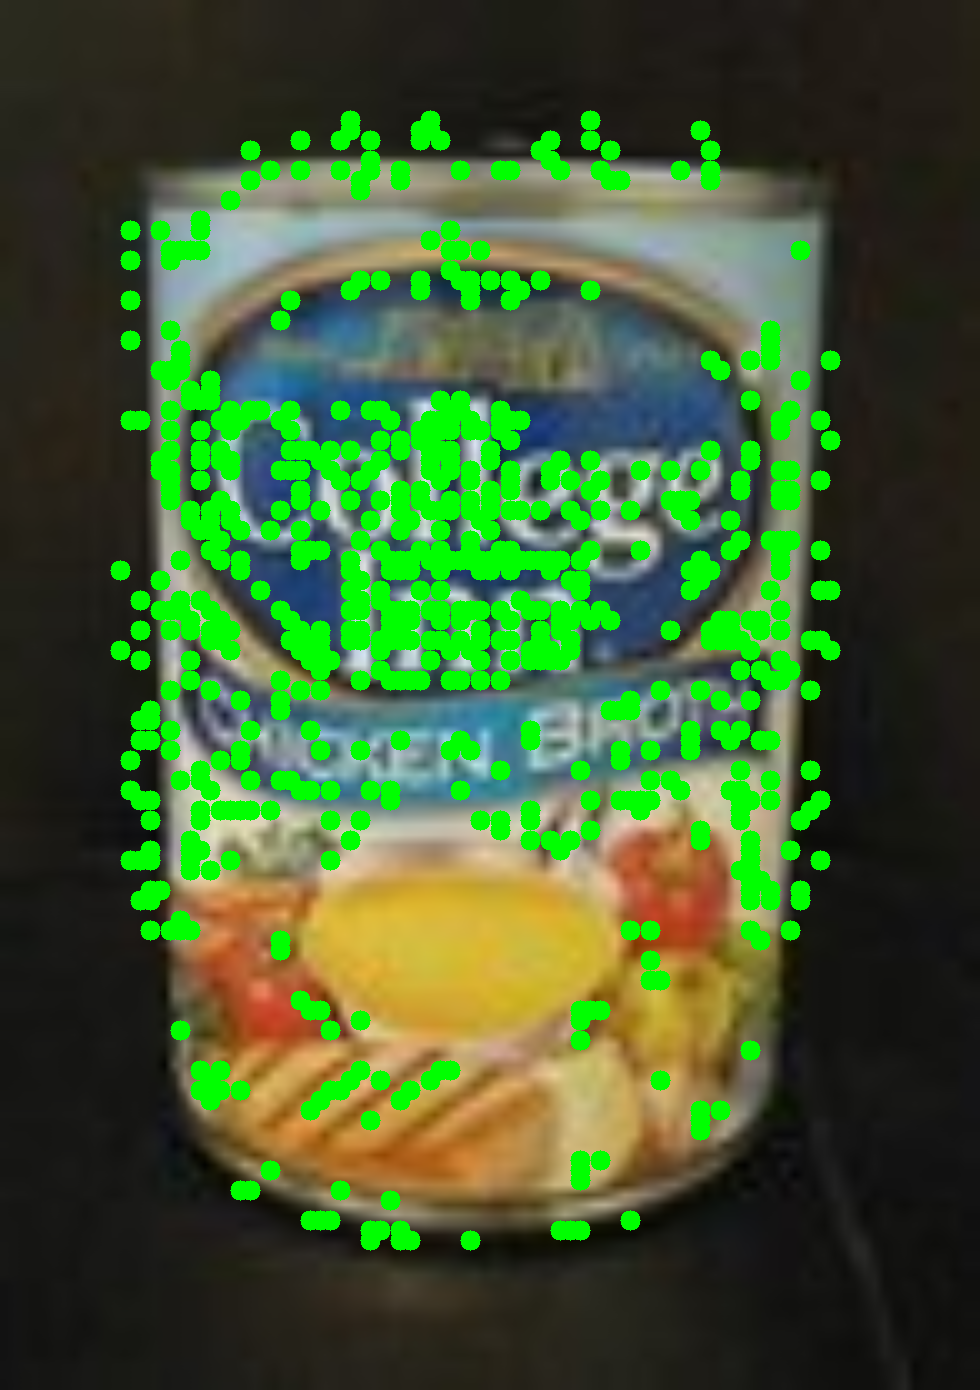
\includegraphics[width=0.45\textwidth]{images/poi_edges}} &
{
\includegraphics[width=0.45\textwidth]{images/poi}}
\end{tabular}
\caption{Keypoint detection without edge suppression (left) and with edge suppression (right)}
\end{figure}

\newpage
\section{BRIEF Descriptor}

\begin{figure}[!ht]
    \centering
    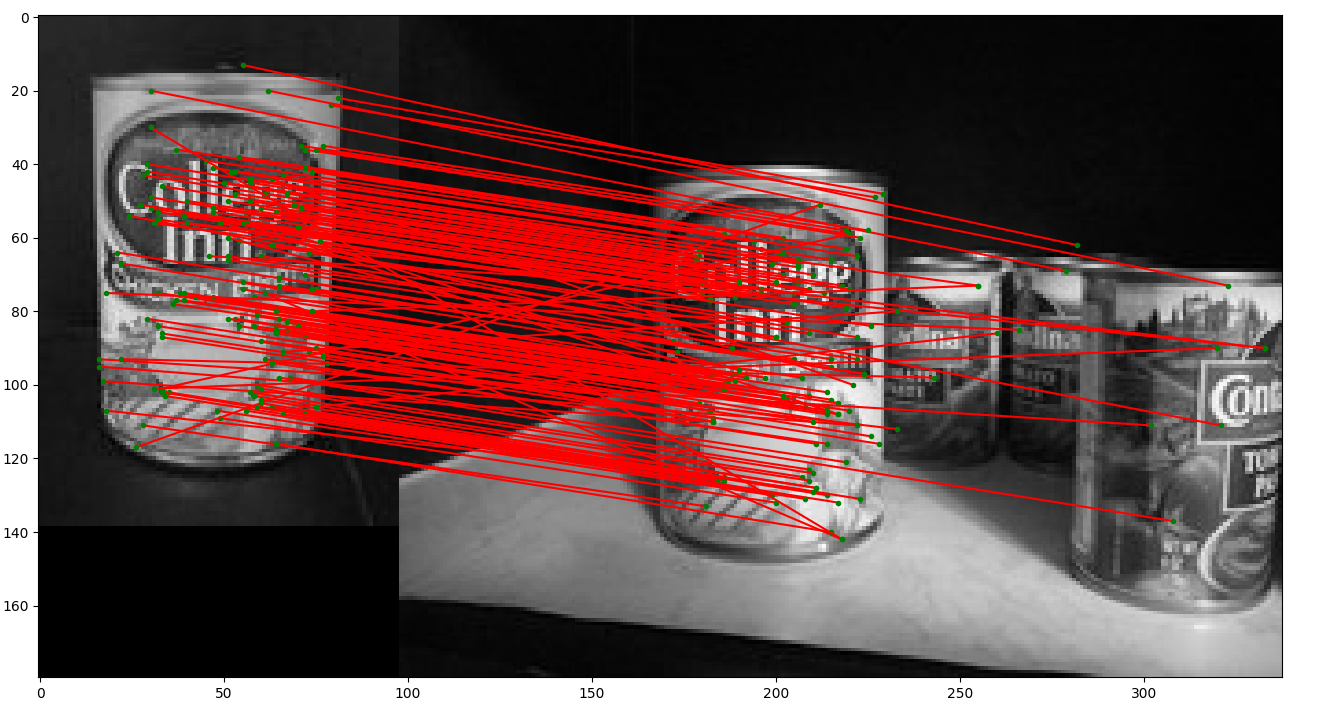
\includegraphics[width=\textwidth]{images/BRIEF_matches}
    \caption{BRIEF matches for \textit{chickenbroth\_01.jpg} and \textit{model\_chickenbroth.jpg}}
\end{figure}

\begin{figure}[!ht]
    \centering
    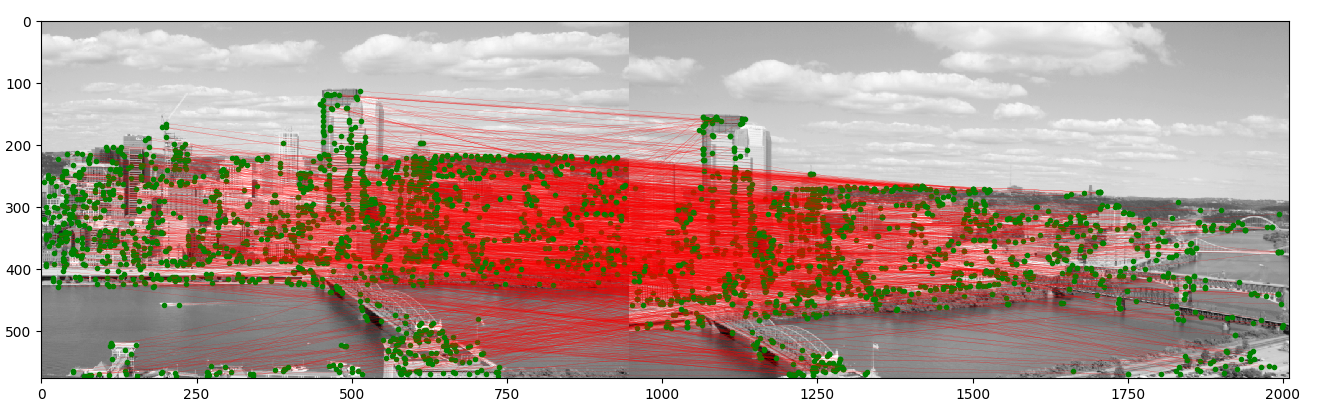
\includegraphics[width=\textwidth]{images/incline_BRIEF}
    \caption{BRIEF matches for \textit{incline\_L.png} and \textit{incline\_R.png}}
\end{figure}

\begin{figure}[!htb]
    \centering
    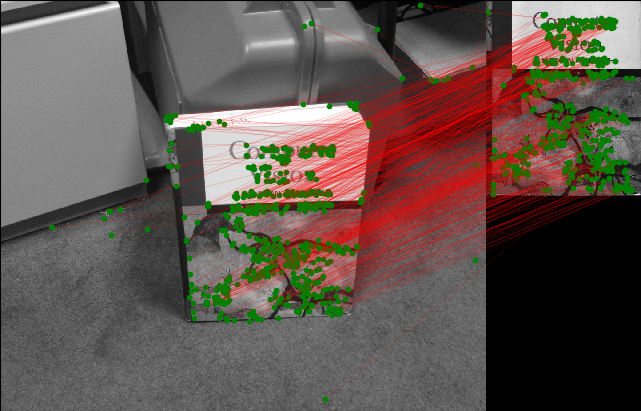
\includegraphics[width=\textwidth]{images/pf_scan_stand}
    \caption{BRIEF matches for \textit{pf\_scan\_scaled.jpg} and \textit{pf\_stand.jpg}}
\end{figure}

\begin{figure}[!htb]
    \centering
    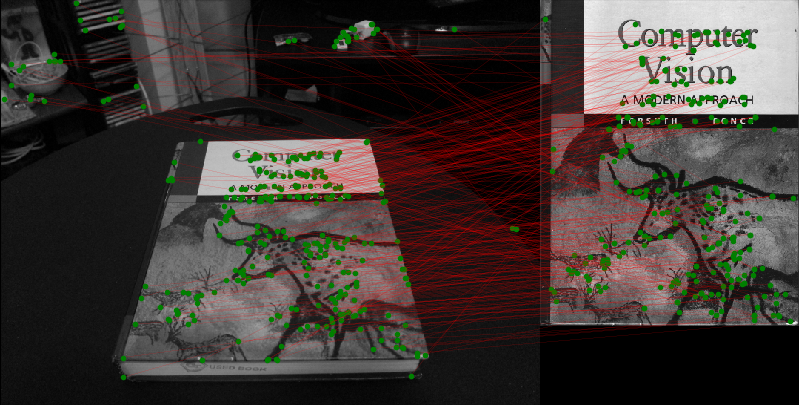
\includegraphics[width=\textwidth]{images/pf_desk}
    \caption{BRIEF matches for \textit{pf\_scan\_scaled.jpg} and \textit{pf\_desk.jpg}}
\end{figure}

\begin{figure}[!htb]
    \centering
    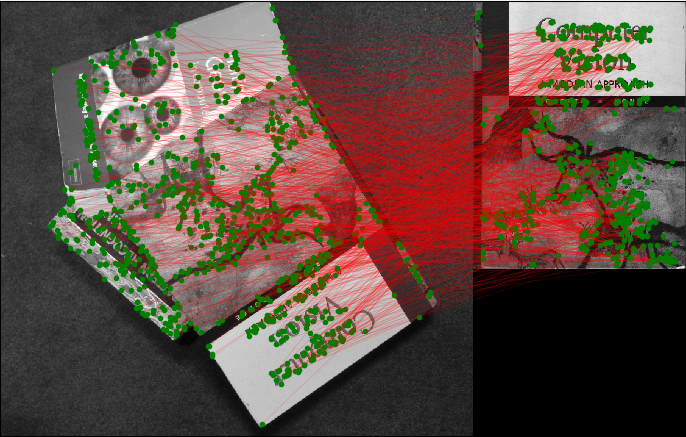
\includegraphics[width=0.8\textwidth]{images/pf_pile}
    \caption{BRIEF matches for \textit{pf\_scan\_scaled.jpg} and \textit{pf\_pile.jpg}}
\end{figure}

\begin{figure}[!htb]
    \centering
    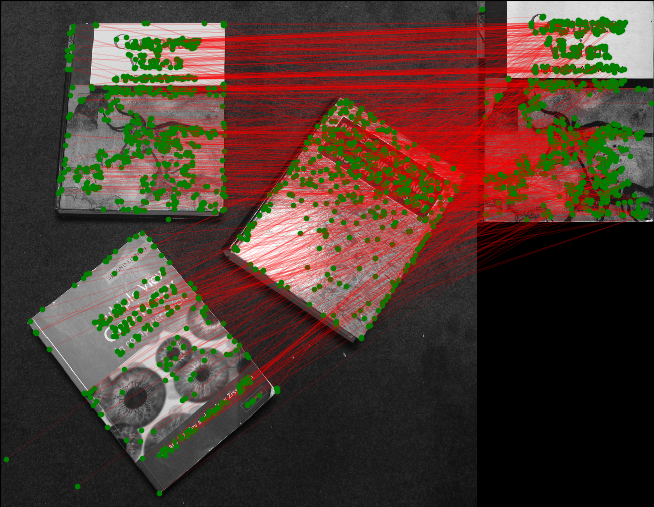
\includegraphics[width=0.8\textwidth]{images/pf_floor}
    \caption{BRIEF matches for \textit{pf\_scan\_scaled.jpg} and \textit{pf\_floor.jpg}}
\end{figure}

\begin{figure}[!htb]
    \centering
    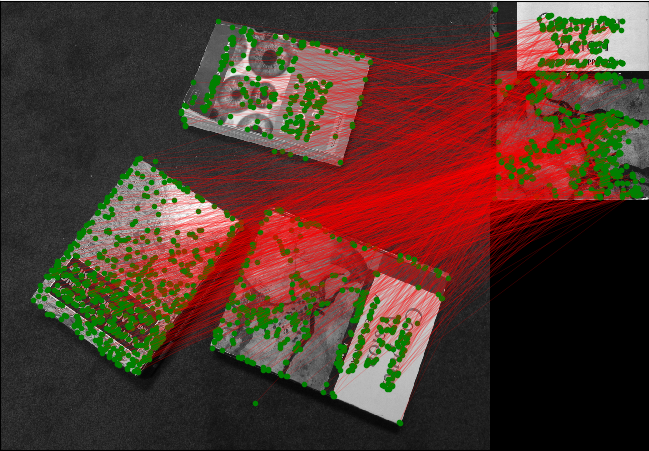
\includegraphics[width=\textwidth]{images/pf_floor_rot}
    \caption{BRIEF matches for \textit{pf\_scan\_scaled.jpg} and \textit{pf\_floor\_rot.jpg}}
\end{figure}

It can be seen from the images that there are a good number of matches using the BRIEF descriptor with some outliers. The result is quite good with some images such as Figures 2, 3 and 4. Figure 7 also has good matches, however it has a lot of outliers probably due to similar keypoints detected from the other books. With Figures 6 and 8, where the book is rotated, the BRIEF matches are very bad with very few correct matches or corresponding points. This is obviously due to the reason that BRIEF is not designed for rotation invariance.\\

The histogram for rotation and number of matches is shown in Figure 9. The histogram plot is as expected. This is because in BRIEF we only select a bunch of random points and compare their intensities within the patch to create a binary descriptor. Although we are selecting keypoints over different scales using Gaussian Pyramids, nowhere are we selecting or taking care of their rotation information. It can be seen from the histogram that after around 10 degrees of rotation, there is a sudden drop in number of matches. Since we are selecting points randomly in the patch, there is a slight increase in matches at 180 degrees. To get better number of matches, our descriptor also should encode some sort of rotation information.

\begin{figure}[!htb]
    \centering
    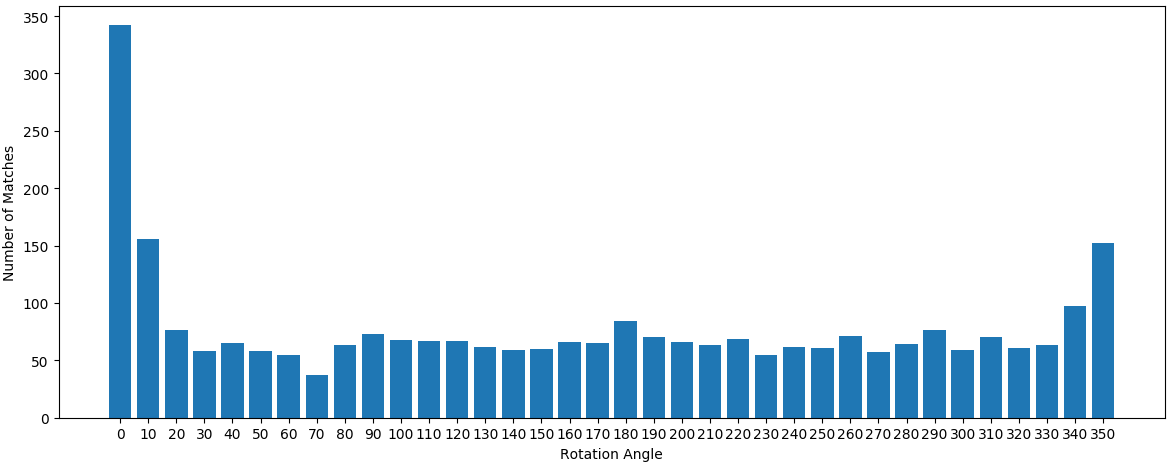
\includegraphics[width=\textwidth]{images/rotation_matches_histogram}
    \caption{Histogram for number of BRIEF matches and rotation angle for \textit{model\_chickenbroth.jpg}}
\end{figure}

\clearpage
\section{Planar Homographies: Theory}

\textbf{a)} Let $\mathbf{\tilde{x_i}} = \begin{bmatrix}
  x_i \quad y_i \quad 1
\end{bmatrix}^\top$ be the set of projected 2D points on the first camera and 
$\mathbf{\tilde{u_i}} = \begin{bmatrix}
  u_i \quad v_i \quad 1
\end{bmatrix}^\top$ be the set of projected 2D points on the second camera.

For $\mathbf{N}$ correspondence points, the homography between these two views is given as follows.
\begin{gather}
\lambda_i\mathbf{\tilde{x_i}} = \mathbf{H}\mathbf{\tilde{u_i}} \quad for \quad i=1:N 
\end{gather}

For any two given points, we can write the above in a matrix form as follows.
\begin{gather}
    \lambda
    \begin{bmatrix}
    x \\ y \\ 1
    \end{bmatrix} = 
    \begin{bmatrix}
  h_{11} & h_{12} & h_{13} \\
  h_{21} & h_{22} & h_{23} \\
  h_{31} & h_{32} & h_{33}
 \end{bmatrix}
    \begin{bmatrix}
    u \\ v \\ w
    \end{bmatrix}
\end{gather}

From the matrix above, we can derive the following relations between $\mathbf{\tilde{x}}$ and $\mathbf{\tilde{u}}$. For inhomogeneous coordinates, $x'=x/\lambda, \quad y'=y/\lambda$.
\begin{gather}
    x' = \frac{h_{11}u + h_{12}v + h_{13}w}{h_{31}u + h_{32}v + h_{33}w}
\end{gather}
\begin{gather}
    y' = \frac{h_{21}u + h_{22}v + h_{23}w}{h_{31}u + h_{32}v + h_{33}w}
\end{gather}

With loss of generality, setting $w=1$ and simplifying the terms above,
\begin{gather}
    x'(h_{31}u + h_{32}v + h_{33}) = h_{11}u + h_{12}v + h_{13}
    \\
    y'(h_{31}u + h_{32}v + h_{33}) = h_{21}u + h_{22}v + h_{23}
\end{gather}

Rearranging the above equations,
\begin{gather}
    x'h_{31}u + x'h_{32}v + x'h_{33} - h_{11}u - h_{12}v - h_{13} = 0
    \\
    y'h_{31}u + y'h_{32}v + y'h_{33} - h_{21}u - h_{22}v - h_{23} = 0
\end{gather}

In the above equation, we have 9 unknowns and a single pair of points just gives us 2 equations. However, $H_{33}$ is a scaling factor and we can normalize the matrix by dividing every other element in $\mathbf{H}$. Now we still have 8 unknowns to find. Therefore, in order to solve this, we will require a minimum of 4 points which will give us 8 equations. In general, we can formulate 2N equations using N points. The following matrix can be formed by stacking each of the 2 equations from all the points,
\begin{gather}
\begin{bmatrix}
-u_1 & -v_1 & -1 & 0 & 0 & 0 & u_1x_1' & v_1x_1' & x_1' \\
0 & 0 & 0 & -u_1 & -v_1 & -1 & u_1y_1' & v_1y_1' & y_1' \\
-u_2 & -v_2 & -1 & 0 & 0 & 0 & u_2x_2' & v_2x_2' & x_2' \\
0 & 0 & 0 & -u_2 & -v_2 & -1 & u_2y_2' & v_2y_2' & y_2' \\
\vdots & \vdots & \vdots & \vdots & \vdots & \vdots & \vdots & \vdots & \vdots & \\
-u_N & -v_N & -1 & 0 & 0 & 0 & u_Nx_N' & v_Nx_N' & x_N' \\
0 & 0 & 0 & -u_N & -v_N & -1 & u_Ny_N' & v_Ny_N' & y_N' \\
\end{bmatrix}
\begin{bmatrix}h_{11} \\ h_{12} \\ h_{13} \\ h_{21} \\ h_{22} \\ h_{23} \\ h_{31} \\ h_{32} \\h_{33} \end{bmatrix} = 0
\end{gather}

We can write this in the form below, where h is a vector of the elements of $\mathbf{H}$ and $\mathbf{A}$ is a matrix composed of elements derived from the point coordinates.
\begin{gather}
    \mathbf{Ah} = 0
\end{gather}

\textbf{b)} As it can be seen in equation 10, $\mathbf{h}$ has 9 elements.\\

\textbf{c)} As explained in the previous section, we need a minimum of 4 points to solve this system. 

Homography has 8 degrees of freedom, despite having 9 elements. This is because the last element or the scaling factor does not contribute to a new degree of freedom. Scaling all the nine elements will cancel out the common factor in equations 3 and 4. 

Each point correspondence gives us 2 equations to help solve this system. \\

\textbf{d)} We need to solve the problem of minimizing the error while estimating $\mathbf{H}$. We can add and extra constraint $|H|=1$ to avoid the obvious solution of $H$ being all zeros. We can solve this using Singular Value Decomposition (SVD).
\begin{gather}
A = USV^\top
\end{gather}

In Python, we can use \textit{np.linalg.svd}, where the singular values will be in descending order. In order to find the $\mathbf{h}$ that best fits all the points, we can take the last singular vector from $\mathbf{V}$ corresponding to the lowest singular value from $\mathbf{S}$. Finally we can reshape it to get $\mathbf{h}$. This gives us a DLT (direct linear transform) homography that minimizes algebraic error and the estimated homography may not be as good as the error does not have a geometric meaning.

\section{Planar Homographies: Implementation}
Implemented in \textit{planarH.py}.

\section{RANSAC}
\begin{figure}[!ht]
    \centering
    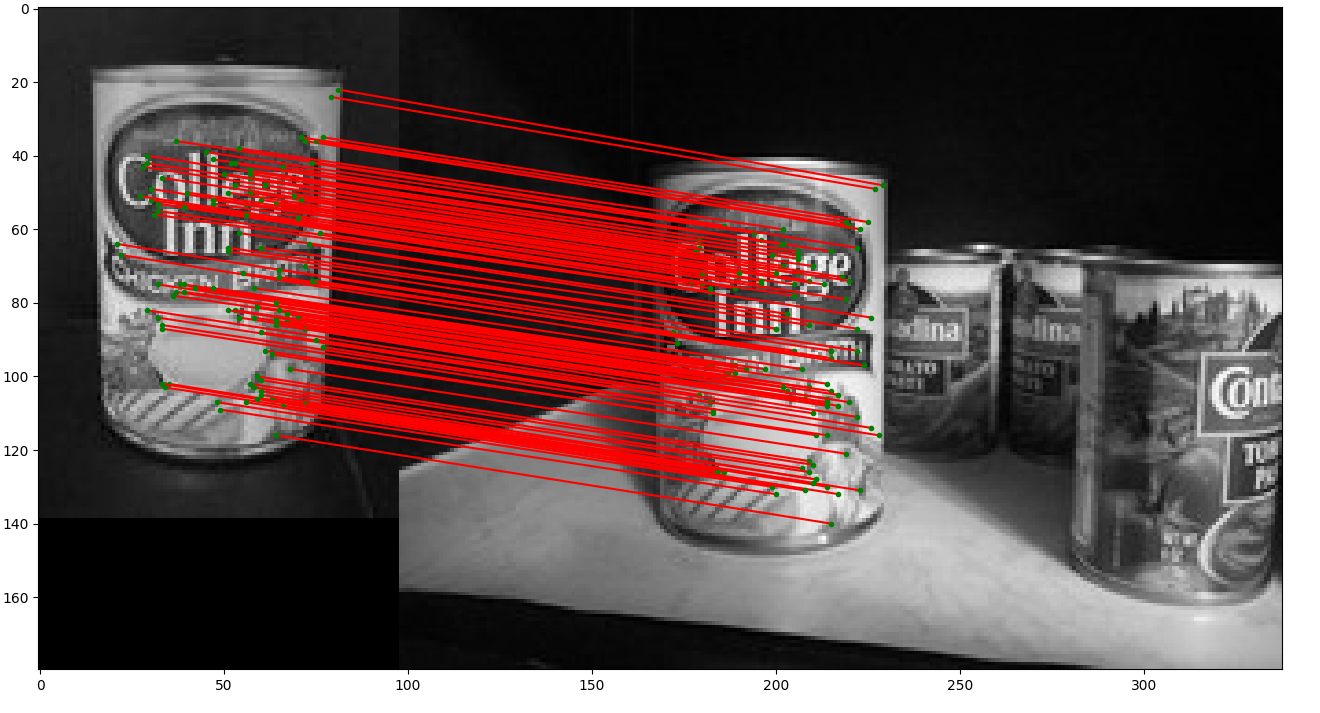
\includegraphics[width=\textwidth]{images/BRIEF_matches_RANSAC}
    \caption{Matches after using RANSAC to remove the outliers for \textit{model\_chickenbroth.jpg} and \textit{chickenbroth\_01.jpg}}
\end{figure}

\begin{figure}[!ht]
    \centering
    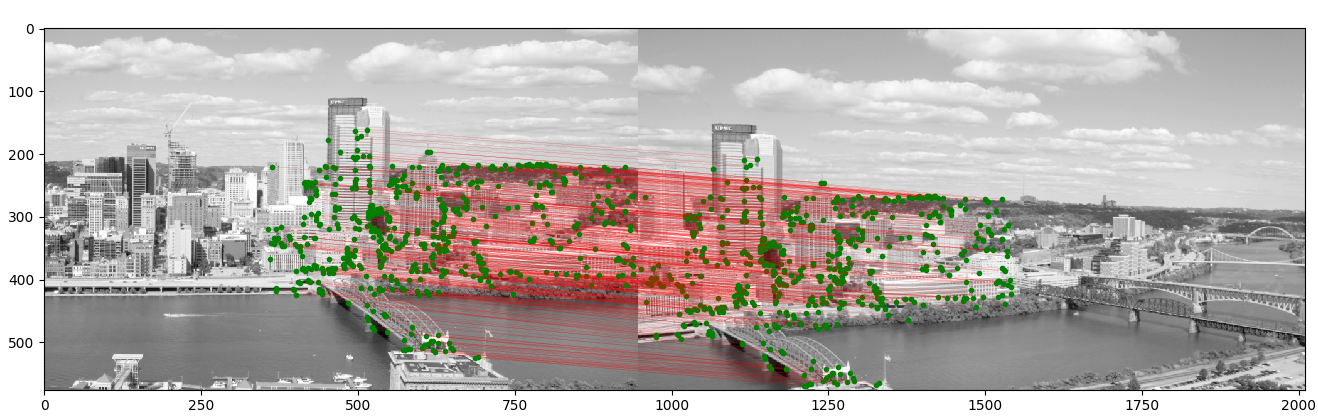
\includegraphics[width=\textwidth]{images/incline_RANSAC}
    \caption{Matches after using RANSAC to remove the outliers for \textit{incline\_L.png} and \textit{incline\_R.png}}
\end{figure}

\section{Stitching it Together: Panoramas}

\begin{figure}[!ht]
    \centering
    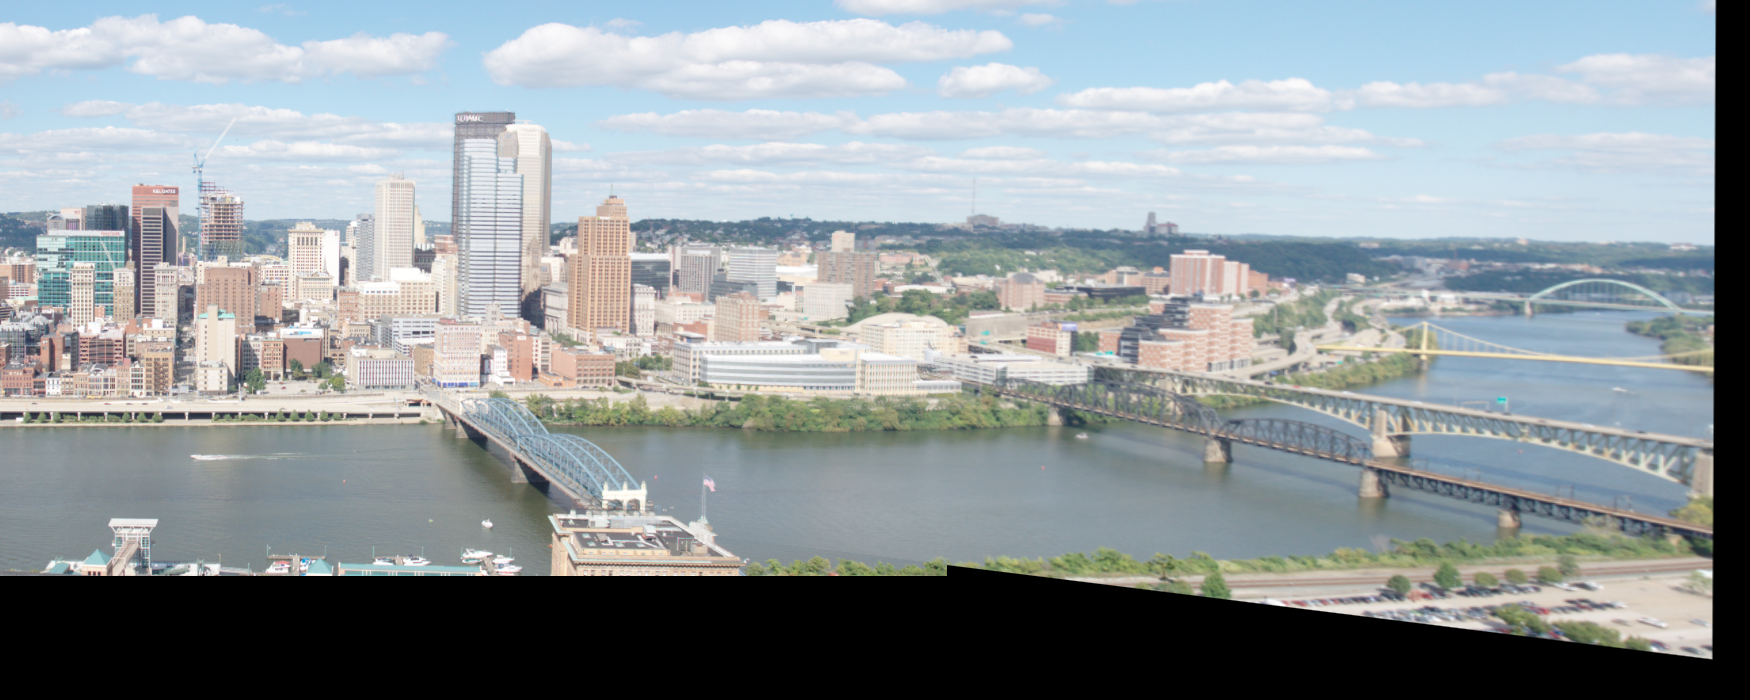
\includegraphics[width=0.95\textwidth]{images/pano_clip}
    \caption{Stitched panorama of Dusquesne Incline (with clipping)}
\end{figure}

\begin{figure}[!ht]
    \centering
    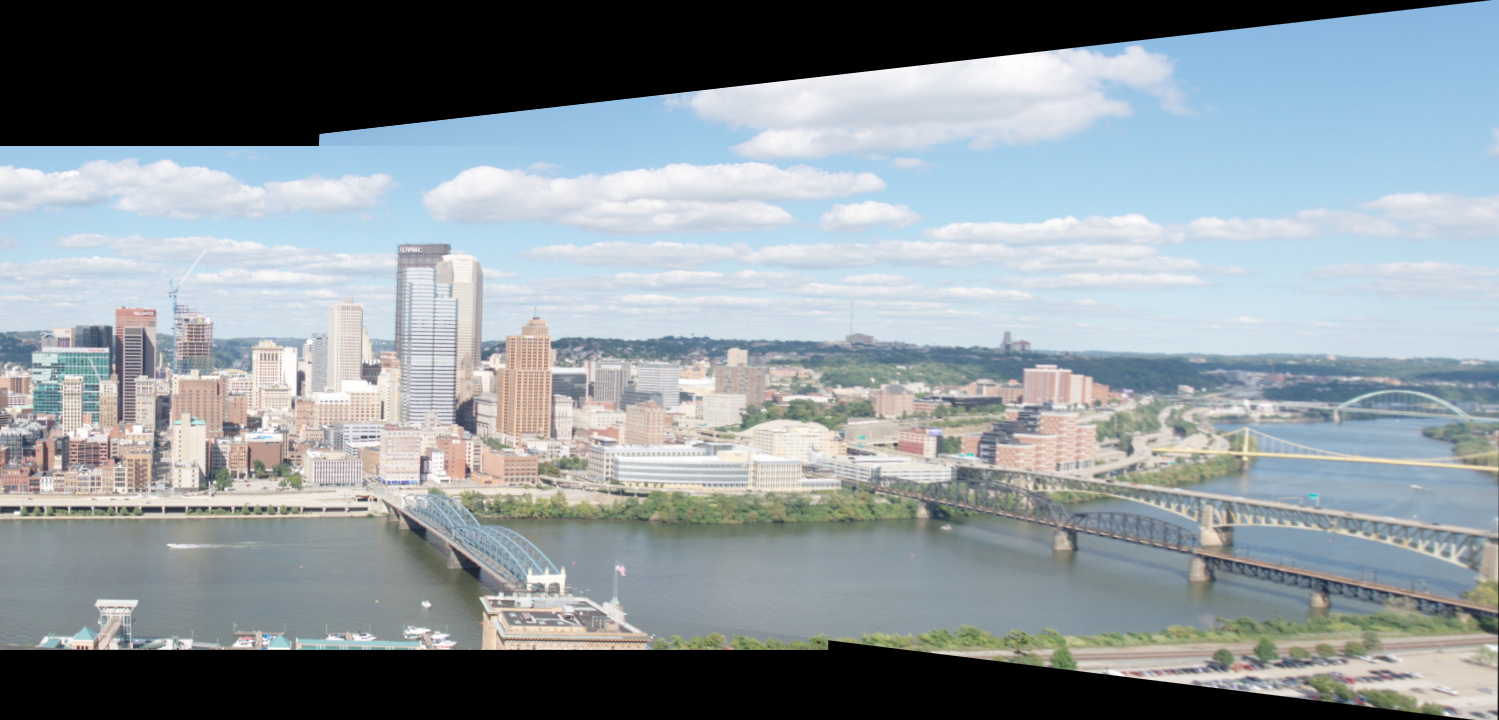
\includegraphics[width=0.95\textwidth]{images/pano_noclip}
    \caption{Stitched panorama of Dusquesne Incline (without clipping)}
\end{figure}

\clearpage
\section{Augmented Reality}

Implemented in \textit{augmented\_reality.py}. Just run the script to display the projected sphere on the image.

\begin{figure}[!ht]
\centering
\begin{tabular}{cc}
{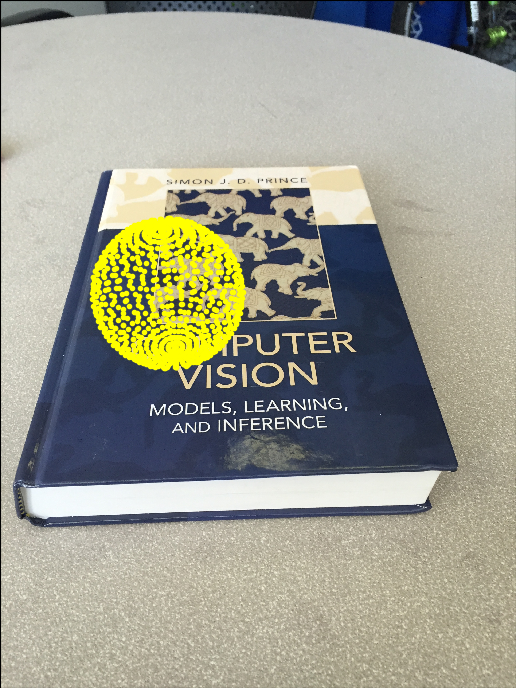
\includegraphics[width=0.45\textwidth]{images/ar_ball}} &
{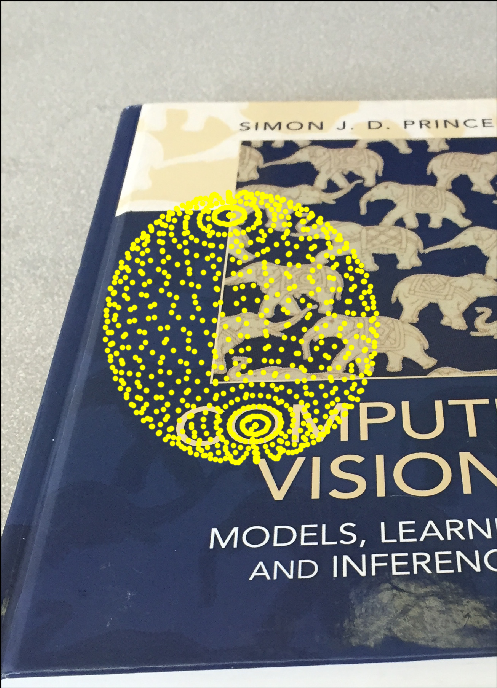
\includegraphics[width=0.45\textwidth]{images/ar_ball_zoom}}
\end{tabular}
\caption{The 3D sphere projected on the 2D plane, centered at 'O' of 'Computer'}
\end{figure}

\end{document}